\documentclass[11pt, oneside]{article} 
\usepackage{geometry}
\geometry{letterpaper} 
\usepackage{graphicx}
	
\usepackage{amssymb}
\usepackage{amsmath}
\usepackage{parskip}
\usepackage{color}
\usepackage{hyperref}

\graphicspath{{/Users/telliott/Github/calculus_book/png/}}
% \begin{center} \includegraphics [scale=0.4] {gauss3.png} \end{center}

\title{Frustum}
\date{}

\begin{document}
\maketitle
\Large

\label{sec:Frustum}

A frustum is the (bottom) part of a larger pyramid or cone that remains after the original solid is cut by a horizontal plane and the upper, small pyramid or cone removed.

\begin{center} 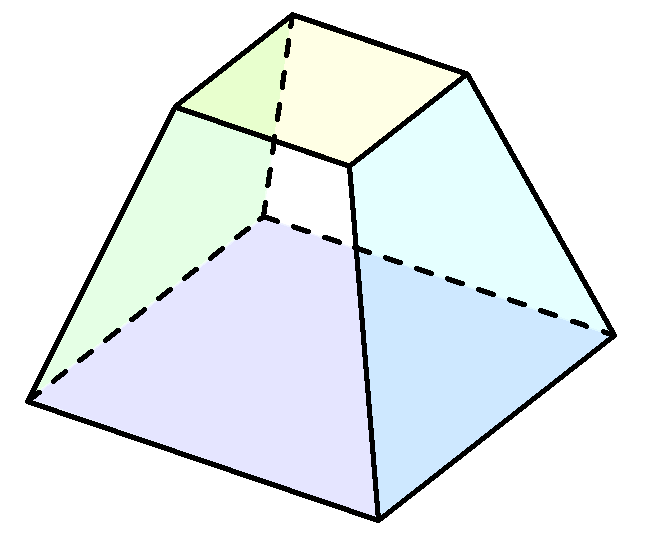
\includegraphics [scale=0.2] {frustum.png} \end{center}

If we call the dimensions of the larger pyramid $H$ (height) and $B$ (base), then its volume is
\[ V = \frac{1}{3} H B^2 \]
Similarly, if we call the dimensions of the pyramid that has been removed $h$ and $b$ its volume is 
\[ V = \frac{1}{3} h b^2 \]

The volume of the frustum is just the difference
\[ V = \frac{1}{3} (H B^2 - h b^2) \]

If we're dealing with a cone rather than a pyramid, then replace $B^2$ with $R^2$ and $b^2$ with $r^2$ and multiply the whole thing by $\pi$.

\subsection*{alternative formula}

However, there is another formula for the volume of the frustum, which is perhaps more interesting.

If we call the altitude or height of the frustum $a$, where $a = H - h$, this formula is
\[ V = \frac{1}{3} a (B^2 + Bb + b^2) \]
\[ V = \frac{1}{3} (H-h) (B^2 + Bb + b^2) \]

We'd like to derive this.  The key insight here is that by similar triangles
\[ \frac{b}{h} = \frac{B}{H},  \ \ \ \ h = \frac{b}{B} H \]
while
\[ a = H - h \]
\[ = H - \frac{b}{B} H \]
\[ = H(1 - \frac{b}{B}) \]
\[ = H (\frac{B - b}{B}) \]

\subsection*{reverse proof}

The proof proceeds easily in the reverse direction.  Start with the answer:
\[  V = \frac{1}{3} a (B^2 + Bb + b^2) \]
Substitute for $a$
\[ V = \frac{1}{3} \ H (1 - \frac{b}{B}) (B^2 + Bb + b^2) \]
Part of this simplifies dramatically
\[ (1 - b/B)( B^2 + Bb + b^2 ) \]
\[ = B^2 + Bb + b^2 - bB - b^2 - \frac{b^3}{B} \]
\[ = B^2- \frac{b^3}{B}  \]

Hence we have that
\[ V = \frac{1}{3} \ H ( B^2 -- \frac{b^3}{B} ) \]
Multiplying out, the first term is $1/3 \ HB^2$, as desired.

The second is
\[ -\frac{1}{3} \ \frac{H}{B} b^3 \]
Recall that $h = bH/B$ so this is just $-1/3 \ hb^2$, and we're done.

$\square$

\subsection*{forward proof}
How would you proceed if you didn't know the answer?  The formula we can easily work out is for the frustrum as the difference in volumes of two pyramids:
\[ V = \frac{1}{3} \ (HB^2 - hb^2) \]

and it's not much of a stretch to substitute for $h=Hb/B$
\[ V = \frac{1}{3} \ (HB^2 - \frac{H}{B}b^3) \]
\[ = \frac{H}{3}  \ (B^2 - \frac{b}{B}b^2) \]
and then since
\[ a = H(1 - \frac{b}{B}) \]
you notice the connection to the previous expression and imagine trying to factor out
\[ (1 - \frac{b}{B})(p + q + r) = (B^2 - \frac{b}{B}b^2) \]

where $p, q$ and $r$ will need to be determined.  Obviously, we will need two sets of cancellations.

We need a term of $B^2$
\[ (1 - \frac{b}{B})(B^2 + q + r ) = (B^2 - \frac{b}{B}b^2) \]
but from $(b/B) \cdot B^2$ we get a term $-bB$ that needs a corresponding term $bB$ from somewhere.  

Similarly we must have a term $b^2$ to generate $b/B \cdot b^2$ so
\[ (1 - \frac{b}{B})(B^2 + q + b^2) = (B^2 - \frac{b}{B}b^2) \]
but then from the $1$ we get a term $b^2$ that needs a corresponding $-b^2$.

Then the inspiration:  $bB$ gives us both of these things.
\[ (1 - \frac{b}{B})(B^2 + bB + b^2) = (B^2 - \frac{b}{B}b^2) \]

I'm not saying it was easy!

Now we just pick up the $(1/3)H$
\[ V = \frac{1}{3}H (1 - \frac{b}{B}) (B^2 + bB + b^2) \] 
 and recall that
\[ a = H(1 - \frac{b}{B}) \]
so
\[ V = \frac{1}{3}a (B^2 + bB + b^2) \]

\subsection*{slant height}
The slant height is the length of a cone or frustum along its outside edge.  In the case of a cone, we can obtain it from the height and $1/2$ the length of the base using the Pythagorean theorem.

For a frustum
\begin{center} 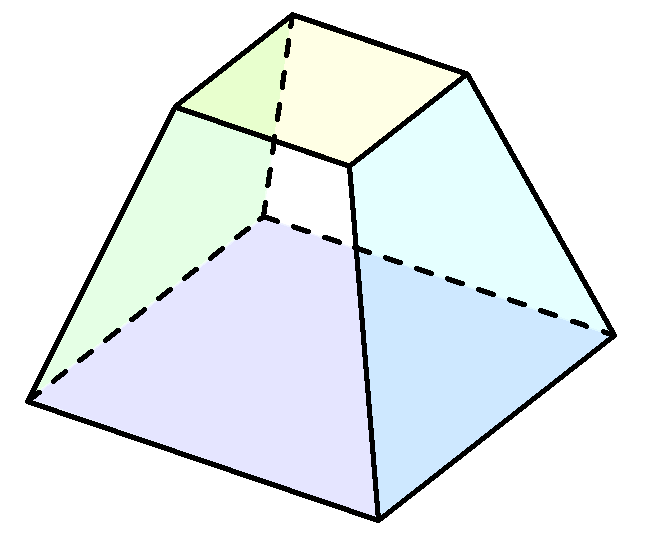
\includegraphics [scale=0.2] {frustum.png} \end{center}
consider the triangle containing an altitude down from the outside edge on the top.

The height of the triangle is just $a$, and the base has length $(B-b)/2$.

If the slant height is $c$ then Pythagoras says that
\[ c^2 = a^2 + (\frac{B - b}{2})^2 \]
\[ a = \sqrt{c^2 - (\frac{B - b}{2})^2} \]


\end{document}  